\documentclass[10pt,landscape]{article}
\usepackage[italian]{babel}
\usepackage[utf8]{inputenc}
\usepackage{multicol}
\usepackage{calc}
\usepackage{ifthen}
\usepackage[landscape]{geometry}
\usepackage{hyperref}
\usepackage{amsmath}
\usepackage{amssymb}
\usepackage{tabularx}
\usepackage{caption}
\usepackage{verbatim}
\usepackage{systeme}
\usepackage{nicefrac}
\usepackage{accents}
\usepackage{enumitem}
\usepackage[printwatermark]{xwatermark}
\usepackage{tikz}
\usetikzlibrary{calc,matrix}
\usepackage[compact]{titlesec}
\usepackage{microtype}
\usepackage[flushleft]{threeparttable}
\usepackage{textcomp}
\usepackage{pifont}
\usepackage{pgfplots}
\usepackage{float}
\usepackage{mathtools}
\usepackage{todonotes}
\usepackage[ruled,vlined]{algorithm2e}

% This sets page margins to .5 inch if using letter paper, and to 1cm
% if using A4 paper. (This probably isn't strictly necessary.)
% If using another size paper, use default 1cm margins.
\ifthenelse{\lengthtest { \paperwidth = 11in}}
{ \geometry{top=.5in,left=.5in,right=.5in,bottom=.5in} }
{\ifthenelse{ \lengthtest{ \paperwidth = 297mm}}
	{\geometry{top=1cm,left=1cm,right=1cm,bottom=1cm} }
	{\geometry{top=1cm,left=1cm,right=1cm,bottom=1cm} }
}

% Turn off header and footer
\pagestyle{empty}

% Reduce size of \section e \subsection
\titleformat{\section}{\normalfont\large\bfseries}{\thesection}{1em}{}
\titleformat{\subsection}{\normalfont\normalsize\bfseries}{\thesubsection}{1em}{}
\titlespacing{\section}{0pt}{0ex}{-0.5ex}
\titlespacing{\subsection}{0pt}{0ex}{-0.5ex}

% Define BibTeX command
\def\BibTeX{{\rm B\kern-.05em{\sc i\kern-.025em b}\kern-.08em
		T\kern-.1667em\lower.7ex\hbox{E}\kern-.125emX}}

% Don't print section numbers
\setcounter{secnumdepth}{0}


\setlength{\parindent}{0pt}
\setlength{\parskip}{0pt plus 0.5ex}

\setlist[itemize]{noitemsep, nolistsep}

% No algorithm numbering
\renewcommand{\thealgocf}{}
% do-while
\SetKwRepeat{Do}{do}{while}

\newcommand{\rarr}{\rightarrow}

\newcommand{\cmark}{\ding{51}}%
\newcommand{\xmark}{\ding{55}}%


\newwatermark[allpages,color=black!10,angle=45,scale=6,xpos=-20,ypos=15]{DRAFT}

\begin{document}

\raggedright
\footnotesize
\begin{multicols}{3}

% multicol parameters
% These lengths are set only within the two main columns
%\setlength{\columnseprule}{0.25pt}
\setlength{\premulticols}{1pt}
\setlength{\postmulticols}{1pt}
\setlength{\multicolsep}{1pt}
\setlength{\columnsep}{2pt}

{\Large{\textbf{Formal Languages and Compilers}}}

\section{Closure Properties}

Let $L \in CF$, $D \in DET$, and $R \in REG$

\begin{table}[H]
    \centering
    \begin{tabularx}{\textwidth}{| r | r | r |}
        $R^R \in REG$ & $L^R \in CF$ & $D^R \notin DET$ \\
        $R^* \in REG$ & $L^* \in CF$ & $D^* \notin DET$ \\
        $\neg R \in REG$ & $\neg L \notin CF$ & $\neg D \in DET$ \\
        $R \cup R \in REG$ & $L \cup L \in CF$ & $D_1 \cup D_2 \notin DET$ \\
        & & $D \cup R \in DET$ \\
        $R . R \in REG$ & $L . L \in CF$ & $D_1.D_2 \notin DET$ \\
        & & $D.R \in DET$ \\
        $R \cap R \in REG$ & $L \cap L \notin CF$ & $D \cap D \notin DET$ \\
        & $L \cap R \in CF$ & $D \cap R \in DET$ \\
    \end{tabularx}
\end{table}

\section{Types of Rules}

\begin{table}[H]
    \centering
    \begin{tabularx}{\textwidth}{| l | c |}
        Terminal & $\rarr a | \epsilon$ \\
        Empty & $\rarr \epsilon$ \\
        Initial & $S \rarr$ \\
        Recursive & $A \rarr \alpha A \beta$ \\
        Left-Recursive & $A \rarr A \beta$ \\
        Right-Recursive & $A \rarr \alpha A$ \\
        Left-Right-Recursive & $A \rarr A \alpha A$ \\
        Copy/Categorization & $A \rarr B$ \\
        Linear & $\rarr u A v | w$ \\
        Left-Linear & $\rarr A v | w$ \\
        Right-Linear & $\rarr v A | w$ \\
        Homogeneous Normal & $\rarr A_1\ldots A_n | a$ \\
        Chomsky Normal & $\rarr AB | a$ \\
        Greibach Normal & $\rarr a\sigma | b$ \\
        Operator Normal & $\rarr A a B$ \\
    \end{tabularx}
\end{table}

\section{Reachable nonterminals}

$A$ is reachable iif $S \Rightarrow^* \alpha A \beta$

For finding the reachable nonterminals build the \textbf{produce} graph and visit it from the axiom.

\section{Defined nonterminals}
$A$ is defined iff $L_A(G) \ne \emptyset$.

For finding the defined nonterminals apply the following relations:
\begin{align*}
    D &:= \{ A | (A \rarr u) \in P, u \in \Sigma^*\} \\
    D &:= D \cup \{ A | (A \rarr B_1\ldots B_n) \in P, \land \forall B_i: B_i \in (D \cup \Sigma) \}
\end{align*}

\section{Circular Derivations}

Derivations like $A \Rightarrow^+ A$, are not essential and introduce ambiguity.

\section{Clean Grammars}
A grammar $G$ is clean iif every nonterminal is \textbf{reachable} and every nonterminal is \textbf{defined}.

\section{Useful Languages}

\paragraph{Dyck Language} $S \rarr bSeS | \epsilon$
\paragraph{Math Expressions}
\begin{align*}
    E &\rarr E + T | T \\
    T &\rarr T * F | F \\
    F &\rarr (E) | i
\end{align*}

\section{Ambiguity}

A sentence $x$ of $G$ is ambiguous iff it admits different syntax trees. In that case $G$ is ambiguous. The degree of ambiguity of $x$ is the number of distinct trees of $x$, of $G$ is the maximum over its sentences.

\paragraph{Bilateral Recursions} $E \rarr E + E | i$ becomes $E \rarr i + E | i$.

\paragraph{Left-Right Recurions in different rules} $A \rarr aA | Ab | c$. Remedies: generate using different rules or force an order of derivation.

\paragraph{Union of Languages} If $L_1 \cap L_2 \ne \emptyset$ then $L_1 \cup L_2$ is ambiguous (the intersection has 2 derivations). Remedy: provide disjointed set of rules: $L_1 \cap L_2$, $L_1 \setminus L_2$ and $L_2 \setminus L_1$.

\paragraph{Concatenation of Languages} $G_1 . G_2$ is ambiguous if $\exists x_1 \in L_1, x_2 \in L_2$ such that $x_1 = uv$ with $u \in L_1$ and $x_2 = vz$ with $z \in L_2$: $uvz$ can be $(uv)z$ or $u(vz)$.

\paragraph{Inherent Ambiguity} A language is inherently ambiguous if all its grammar are ambiguous, e.g. those where the intersection is not CF.

\paragraph{Lack of Order in Derivations} $S \rarr bSc | bbSc | \epsilon$ becomes $S \rarr bSc | D$, $D \rarr bbDc | \epsilon$.

\section{Grammar Equivalence}

\paragraph{Weak Equivalence} $G_1$ weakly equivalent to $G_2$ iff $L(G_1) = L(G_2)$ (even with different trees). It is not decidable.

\paragraph{Strong Equivalence} If weak equivalent and same condensed skeleton trees.

Strong $\Rightarrow$ Weak

\section{Grammar Transformations}

\subsection{Expansion of a nonterminal}
Eliminate a nonterminal: $A \rarr \alpha B \gamma$, $B \rarr \beta_1 | \ldots | \beta_n$ becomes $A \rarr \alpha \beta_1 \gamma | \ldots | \alpha \beta_n \gamma$.

It's always possible to remove the axiom from the right part by adding a new axiom $S_0 \rarr S$.

\subsection{Elimination of empty rules}
A nonterminal is \textbf{nullable} iff it exists a derivation $A \Rightarrow^+ \epsilon$.
\begin{align*}
    A \in \text{Null} &\text{ if }A \rarr \epsilon \in P \\
    A \in \text{Null} &\text{ if } A \rarr A_1\ldots A_n \in P, A_i \in V \setminus \{A\} \land \forall A_i (A_i \in \text{Null})
\end{align*}
\textbf{Note}: Recursive rules cannot be used.

\paragraph{Construction of the non-nullable normal form}
\begin{itemize}
    \item Compute the Null set.
    \item For each rule add as alternative all the combinations of removing the nullable nonterminals.
    \item Remove all empty rules ($A \rarr \epsilon$) excpet for $A = S$.
    \item Clean the grammar and remove circularity.
\end{itemize}

\textbf{Example} $S \rarr SAB | AC$, $A \rarr aA | \epsilon$, $B \rarr bB | \epsilon$, $C \rarr cC | c$. Null is $\{A, B\}$, remove $A$ and $B$ from the rules in every combination: $S \rarr SAB | SA | SB | S | AC | C$, $A \rarr aA | a$, $B \rarr bB | b$, $C \rarr cC | c$. Then remove circularity ($S \rarr S$).

\subsection{Elimination of copy rules}
$\text{Copy}(A) = \{ B \in V | A \Rightarrow^* B \}$.

Assuming \textbf{grammar with no empty rules}, apply until a fixed point:
\begin{align*}
    A &\in \text{Copy}(A) \\
    C &\in \text{Copy}(A) \text{ if } B \in \text{Copy}(A) \land B \rarr C \in P
\end{align*}

\paragraph{Construction of the grammar without copy rules}

\begin{itemize}
    \item Remove copy rules: $P' := P \setminus \{A\rarr B | A, B \in P\}$
    \item Add compensating rules: $P' := P' \cup \{ A \rarr \alpha | \exists B (B \in \text{Copy}(A) \land (B \rarr \alpha \in P)) \}$
\end{itemize}

\textbf{Example} $E \rarr E + T | T$, $T \rarr T \times C | C$, $C \rarr 0|\ldots|9$.
$\text{Copy}(E)=\{E,T,C\}$, $\text{Copy}(T) = \{T, C\}$, $\text{Copy}(C) = \{C\}$.
The grammar becomes $E \rarr E+T|T\times C|0|\ldots|9$, $T \rarr T\times C|0|\ldots|9$, $C \rarr 0|\ldots|9$.

\subsection{Conversion from left to right recursion}

\paragraph{Immediate L-recursions} $A \rarr A\beta_1 | \ldots | A\beta_h$ where no $\beta_i$ is empty, $A \rarr \gamma_1 | \ldots | \gamma_k$. Introduce new nonterminal $A'$:
\begin{align*}
    A &\rarr \gamma_1A' | \ldots | \gamma_kA' | \gamma_1 | \ldots | \gamma_k \\
    A' &\rarr \beta_1A' | \ldots | \beta_hA' | \beta_1 | \ldots | \beta_h
\end{align*}

\textbf{Example} $E \rarr E+T | T$, $T \rarr T\times F | F$, $F \rarr (E) | i$. It becomes $E \rarr TE' | T$, $E' \rarr +TE'|+T$, $T \rarr FT'|F$, $T' \rarr \times FT'|\times F$, $F\rarr (E)i$.

\textbf{Non-Immediate L-recurions} are much harder and not covered by the slides.

\section{Unilinear Grammar}

A grammar is unilinear iff all rules are either all left-linear or right-linear. It can also be required that it has:
\begin{itemize}
    \item Strictly unilinear rules: $A \rarr aB$ with $a\in \Sigma \cup \epsilon$ and $B \in V \cup \epsilon$
    \item All terminal rules are empty: $B \rarr b$ replaced with $B \rarr bB'$, $B' \rarr \epsilon$
\end{itemize}

\subsection{From Unilinear to Regular Expression}

\textbf{Assumptions}: strictly right unilinear, all terminal rules empty.

For every nonterminal $A$ defined by $A \rarr a_1A_1|\ldots|a_kA_k|\epsilon$:
$L_A = a_1L_{A_1} \cup | \ldots | \cup a_kL_{A_k} \cup \epsilon$

\textbf{Arden Identity}: $X = KX \cup L$ (with $K$ nonempty) has exactly one solution $X = K^*L$.

\textbf{Example} $S \rarr sS | eA$, $A \rarr sS|\epsilon$
\begin{alignat*}{2}
&
    \begin{cases}
        L_S = sL_S \cup eL_A \\
        L_A = sL_S \cup \epsilon
    \end{cases}
&&
    \begin{cases}
        L_S = sL_S \cup e(sL_S \cup \epsilon) \\
        L_A = sL_S \cup \epsilon
    \end{cases}
\\
&
    \begin{cases}
        L_S = (s \cup es) L_S \cup e \\
        L_A = sL_S \cup \epsilon
    \end{cases}
&&
    \begin{cases}
        L_S = (s \cup es)^*e \\
        L_A = sL_S \cup \epsilon = s(s \cup es)^*e \cup \epsilon
    \end{cases}
\end{alignat*}


\section{Clean Automata}

A state is $q$ \textbf{reachable} from $p$ if there is a computation from $p$ to $q$.
A state is \textbf{accessible} if it is reachable from the initial state.
A state is \textbf{post-accessible} if a final state can be reached from it.
A state is \textbf{useful} if it is accessible and post-accessible.

An automaton is \textbf{clean} if all the states are useful.

\section{Minimal Automaton}

\textbf{Assumption}: the automaton is clean except for the $q_{err}$ state.

State $p$ is indistinguishable from $q$ iff $\forall x, \delta(p,x)$ and $\delta(q, x)$ are both final or non-final. Indistiguishability is an equivalence relation, 2 indistinguishable states can be merged with no change in the language recognized.

\subsection{Compute distinguishability set}
$p$ is distinguishable from $q$ iff
\begin{itemize}
    \item $p$ is final and $q$ is not, or vice-versa; or
    \item $\exists a: \delta(p, a)$ is distinguishable from $\delta(q, a)$
\end{itemize}

\textbf{Example}
\begin{figure}[H]
    \centering
    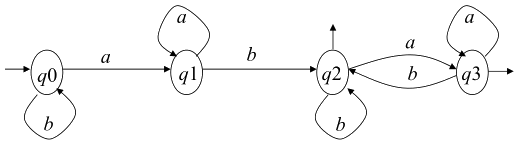
\includegraphics[width=\linewidth]{automata/example-automaton-minimization.png}
\end{figure}

\begin{table}[H]
    \centering
    \begin{minipage}{0.35\linewidth}
        \begin{tabular}{r|c|cc}
            \cline{2-2}
            $q_1$ & & & \\
            \cline{2-3}
            $q_2$ & \xmark & \multicolumn{1}{c|}{\xmark} & \\
            \cline{2-4}
            $q_3$ & \xmark & \multicolumn{1}{c|}{\xmark} & \multicolumn{1}{c|}{} \\
            \cline{2-4}
            \multicolumn{1}{c}{} & \multicolumn{1}{c}{$q_0$} & $q_1$ & $q_2$
        \end{tabular}
    \end{minipage}
    \begin{minipage}{0.6\linewidth}
        \begin{tabular}{r|c|cc}
            \cline{2-2}
            $q_1$ & (1,1)(0,2) & & \\
            \cline{2-3}
            $q_2$ & \xmark & \multicolumn{1}{c|}{\xmark} & \\
            \cline{2-4}
            $q_3$ & \xmark & \multicolumn{1}{c|}{\xmark} & \multicolumn{1}{c|}{(3,3)(2,2)} \\
            \cline{2-4}
            \multicolumn{1}{c}{} & \multicolumn{1}{c}{$q_0$} & $q_1$ & $q_2$
        \end{tabular}
    \end{minipage}
    \begin{minipage}{0.6\linewidth}
        \begin{tabular}{r|c|cc}
            \cline{2-2}
            $q_1$ & \xmark & & \\
            \cline{2-3}
            $q_2$ & \xmark & \multicolumn{1}{c|}{\xmark} & \\
            \cline{2-4}
            $q_3$ & \xmark & \multicolumn{1}{c|}{\xmark} & \multicolumn{1}{c|}{(3,3)(2,2)} \\
            \cline{2-4}
            \multicolumn{1}{c}{} & \multicolumn{1}{c}{$q_0$} & $q_1$ & $q_2$
        \end{tabular}
    \end{minipage}
\end{table}

States $q_2$ and $q_3$ are indistinguishable, so they can be merged.

\begin{figure}[H]
    \centering
    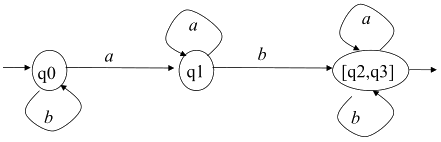
\includegraphics[width=\linewidth]{automata/example-automaton-minimization-2.png}
\end{figure}


\rule{0.3\linewidth}{0.25pt}
\scriptsize\\
\href{mailto:edoardo.morassutto@mail.polimi.it}{Edoardo Morassutto}, Politecnico di Milano, A.A. 2019/2020
\end{multicols}
\end{document}
